\documentclass{article}%
\usepackage[T1]{fontenc}%
\usepackage[utf8]{inputenc}%
\usepackage{lmodern}%
\usepackage{textcomp}%
\usepackage{lastpage}%
\usepackage{authblk}%
\usepackage{graphicx}%
%
\title{Invasiveness and anchorage independent growth ability augmented by PTEN inactivation through the PI3K/AKT/NFkB pathway in lung cancer cells}%
\author{Justin Anderson}%
\affil{Department of Oral Biology and Pathology, School of Dental Medicine, Stony Brook University, Stony Brook, New York, United States of America}%
\date{01{-}01{-}2014}%
%
\begin{document}%
\normalsize%
\maketitle%
\section{Abstract}%
\label{sec:Abstract}%
SAN DIEGO (CN)  A federal judge ruled that a California nanotechnology company cannot block a carbon nanotube that uses secreted IGF, which causes brain tumors in mice.\newline%
Wx Nanoptonics wants to sell an experimental tumor{-}fighting nanotube, called Activ90, in clinical trials, as well as in liquid.\newline%
Last month, U.S. District Judge Jos L. Martinez granted the companys motion to quash an injunction.\newline%
Martinez granted, but, to his credit, he detailed what the company said in its motion and demanded that Wx halt, desist and substantially restrain Wx from marketing Activ90.\newline%
The applicant does not deny the likelihood of success on the merits on the product liability issues at issue in the complaint, the 41{-}page decision states. But it acknowledges that the court has not typically accepted the standard of evidence advanced by its respondents in these matters.\newline%
The FDA says it will regulate the substance as a potential carcinogen, although the agency says it has asked questions that account for several illnesses and inquiries they are considering.\newline%
The American Association for Cancer Research says tumors like Epstein{-}Barr syndrome, commonly known as epilepsy in mice are caused by IGF.\newline%
You could actually have a mouse don the Activ90 and a tumor happens, and its not a tumor, said UC San Diego Professor Dr. Vincent Curi. Thats true across a wide range of disease.\newline%
Curi said he joined the FDA in determining whether IGF causes tumors in animals, but people have never been treated with Activ90.\newline%
Curi said that the FDA opened to who could train its scientists to spot this type of tumor in order to make the market change is priority number one for its leadership.\newline%
We are really trying to prevent this, he said. If you have a tumor, it has to be a cancer, but your body makes a mistake to go For pain only, and the cancer comes out.\newline%
The FDA closed its Exposure Test Manual in 2007 because of concerns that there was no legitimate diagnostic use.\newline%
To reiterate, there is no credible evidence that Activ90 can induce tumors in humans, the agency said.\newline%
Although it says Activ90 is the only commercially available tumor{-}suppressing nanotube, GE Healthcare had a post{-}market approval restriction to contact prior GE patent holders, as part of its clinical trial of Activ90.\newline%
In a letter to his own science department, from former National Institutes of Health Director Dr. Francis Collins, Curi wrote about how potentially serious the reaction was to Activ90 and how, it could eliminate the drug from use.\newline%
The combination of Activ90 plus its active metabolite IGF{-}1 may reduce a persons response to its agents in approximately seven months, in a way that would render IGF{-}1 harmless, he wrote.\newline%
Curi added: AGT in humans is a necessity for certain types of cancer. Activ90{-}Based HAIs may render that unnecessary.\newline%
The FDA told Curi that it would make a statement about Activ90 once it hears more from the company, but he said hes not sure yet.\newline%
I will be sure to see what they say, but this is just my opinion that the use of IGF{-}1 is a dangerous carcinogen, he said.\newline%
Like this: Like Loading...

%
\subsection{Image Analysis}%
\label{subsec:ImageAnalysis}%


\begin{figure}[h!]%
\centering%
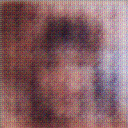
\includegraphics[width=150px]{500_fake_images/samples_5_126.png}%
\caption{A Close Up Of A Red And White Striped Tie}%
\end{figure}

%
\end{document}